% ----------------------------------------------------------------------------
\begin{titlepage}
% ---------------
\begin{center}
{\LARGE\sc Association Terre Virtuelle}\\
\vspace{2cm}
\mbox{\LARGE \sc Projet NaVisu}\\
\vspace{1cm}
\href{https://github.com/terre-virtuelle/navisu.git}{https://github.com/terre-virtuelle/navisu.git}\\
\vspace{2cm}
\mbox{\LARGE \sc Dossier de d�veloppement}\\
\vspace{1cm}

\begin{bfseries}

\begin{Huge}
\soustitre
\end{Huge}

\vspace{.8cm}

\null\vfill

%%%%%%%%%%%%%%%%%%%%%%%%%%%%%%%%%%%%%%%%%%%%%%%%%%%%%%%%%%%%%%%%%%%%%%

\begin{center}
	 \href{https://github.com/terre-virtuelle/navisu.git}{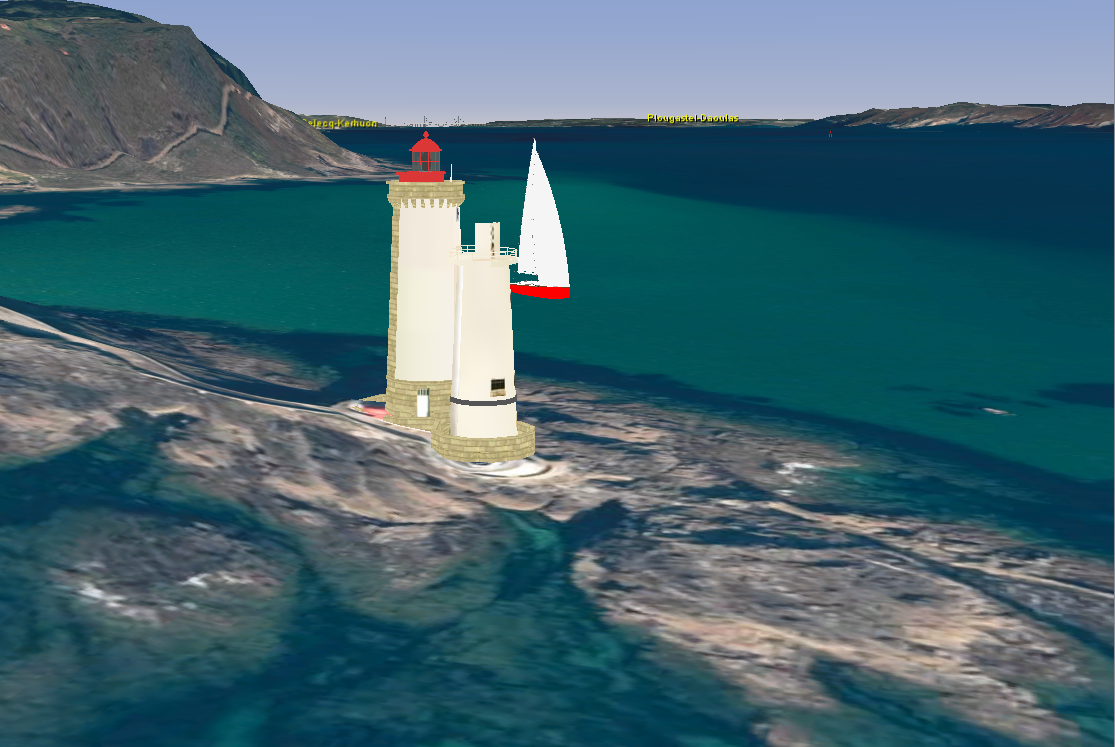
\includegraphics[width=16cm]{images/leMinou.png}}
\end{center}

%%%%%%%%%%%%%%%%%%%%%%%%%%%%%%%%%%%%%%%%%%%%%%%%%%%%%%%%%%%%%%%%%%%%%%%
\null\vfill

\vspace{1cm}
2016

\end{bfseries}
\end{center}

\end{titlepage}

\hbox{}
\newpage
% -------------------

% --- Tracabilite du document
\section*{Tra\c cabilit\'e du document}
\section*{R\'edaction}


\section*{Personnes ayant particip\'ees au projet}

\begin{tabular}{|l|} \hline
Noms \\
\hline
3dphi \\
jojal29 \\
lithops \\
mhyrdin \\
tibus29 \\
\hline
\end{tabular}



\section*{Historique des \'evolutions}

\begin{tabular}{|l|l|} \hline
Version         & Date        \\ 
\hline 
   1.0         &   mai 2015  \\
\hline 
   1.1         &   \ladate   \\
\hline
\end{tabular}

\vfill
\vspace{1cm}{\em Image de couverture : Entr�e du goulet de Brest, le phare du
petit Minou (France)}

\newpage
\hbox{}
\newpage


% --- Table des matieres ---
\tableofcontents

\hbox{}
\newpage

% --- Table des figures ---
\listoffigures

\newpage
\hbox{}
\newpage